
% Modelo de Trabalho Acadêmico da UNESP de Guaratinguetá v-2.1
% atualização Copyright 2024 by Biblioteca FEG UNESP com colaboração de Vitor Pinto Ribeiro and Gustavo Santos Borges and Ronaldo César de Paiva
% Modelo de Trabalho Acadêmico da UNESP de Guaratinguetá v-1.0
% original copyright 2017 by Eduardo Rohde Eras

% This program is free software: you can redistribute it and/or modify
% it under the terms of the GNU General Public License as published by
% the Free Software Foundation, either version 3 of the License, or
% (at your option) any later version.
%
% This program is distributed in the hope that it will be useful,
% but WITHOUT ANY WARRANTY; without even the implied warranty of
% MERCHANTABILITY or FITNESS FOR A PARTICULAR PURPOSE.  See the
% GNU General Public License for more details.
%
% You should have received a copy of the GNU General Public License
% along with this program.  If not, see <http://www.gnu.org/licenses/>.
%
%----------------------------------------------------------------------------------------%
%APRESENTAÇÃO 
% Este modelo pode ser usado como apoio para seu trabalho acadêmico e é destinado para ser usado no Word, não aplicável a outros editores de texto.
%
%Essas instruções são voltadas para a comunidade acadêmica da Universidade Estadual Paulista “Júlio de Mesquita Filho” (Unesp). Caso você seja de outra instituição, verifique as regras vigentes da sua universidade ou faculdade.
%
%O uso deste modelo não substitui o conhecimento das normas, diretrizes da universidade e orientações de seus professores e a Rede de Bibliotecas da Unesp está isenta de eventuais e quaisquer problemas ou prejuízos decorrentes do uso deste arquivo em softwares não licenciados, arquivos corrompidos, vírus ou quaisquer outros motivos.
%
%Em caso de dúvidas, consulte o Manual de normalização de trabalhos acadêmicos: apresentação: ABNT (2023): \url{https://docs.google.com/document/d/1ipkGiAUnAr_YBTrpFJpnud3aa4llBsROpBdkUfw91L0/edit?usp=sharing}
%----------------------------------------------------------------------------------------%
% C L A S S E   D O   D O C U M E N T O
%----------------------------------------------------------------------------------------%

\PassOptionsToPackage{colorlinks=true, allcolors=black}{hyperref}
\documentclass[
  %----------------------------------------------------------------------------------------%
  %Opções da classe 'memoir'
  %----------------------------------------------------------------------------------------%
  12pt,		% Tamanho da Fonte.
  a4paper,	% Tamanho da página.
  openright,  % Capítulos começam em páginas ímpares (insere uma página vazia se necessário).
  oneside,	% Para impressão em frente e verso utilizar twoside.
  %----------------------------------------------------------------------------------------%
  %Opções da classe 'abntex2'
  %----------------------------------------------------------------------------------------%
  chapter=TITLE,		%Títulos de capítulos convertidos em letras maiúsculas.
  section=TITLE,		%Títulos de seções convertidos em letras maiúsculas.
  %----------------------------------------------------------------------------------------%
  %Opções da classe 'babel'
  %----------------------------------------------------------------------------------------%
  english,	%Idioma adicional para hifenização.
  french,	    %Idioma adicional para hifenização.
  spanish,	%Idioma adicional para hifenização.
  brazil	    %Idioma principal do documento.
  %----------------------------------------------------------------------------------------%
]{abntex2}

%----------------------------------------------------------------------------------------%
% P A C O T E S
%
% Insira aqui os pacotes que for utilizar em seu documento. Para saber quais pacotes o
% template já está utilizando, confira o arquivo "pacoteBasico.sty".
%----------------------------------------------------------------------------------------%
    
    \usepackage{pacoteBasico}   %Pacote Básico de formatação no padrão da UNESP/FEG
    \usepackage{color}		    %Controle das cores.
    \usepackage{graphicx}	    %Inclusão de gráficos.
    \usepackage{lipsum}		    %Para geração de 'Dummy Text'.
    \usepackage{pdfpages}       %Para inclusão de arquivos pdf
    \usepackage[table,xcdraw]{xcolor}


    
%----------------------------------------------------------------------------------------%
% I N F O R M A Ç Õ E S   B Á S I C A S   S O B R E   O   T R A B A L H O
%
% Defina aqui as informações pertinentes ao trabalho.
%----------------------------------------------------------------------------------------%

%----------------------------------------------------------------------------------------%
% D A D O S   P E S S O A I S
%----------------------------------------------------------------------------------------%

%Nome completo do autor do presente Trabalho acadêmico:
\newcommand{\nomeDoAutor}{
	Jonas Ernesto Poli
}

%Nome do curso:
\newcommand{\nomeDoCurso}{Programa de Pós Graduação em Ciência, Tecnologia e Sociedade}

%----------------------------------------------------------------------------------------%
% D A D O S   S O B R E   O   T R A B A L H O
%----------------------------------------------------------------------------------------%

%Título do presente trabalho:
\newcommand{\tituloDoTrabalho}{
	Título do trabalho acadêmico
}

%Subtítulo do presente trabalho, se houver:
\newcommand{\subtituloDoTrabalho}{
	subtítulo se houver
}

%Tipo do trabalho (Dissertação / Tese / Trabalho de Conclusão de Curso / Trabalho de Conclusão de Residencia) 
\newcommand{\tipoDeTrabalho}{Tipo de Trabalho Acadêmico}

% Nome da Faculdade ou instituto
\newcommand{\NomeDaFaculdade}{UFSCAR}

%Grau acadêmico (Mestre(a) / Doutor(a) / Bachareal / Licenciatura etc)
\newcommand{\GrauAcademico}{Mestre}

% área de concentração, se houver (muito utilizado no mestrado e doutorado) % remover no pacote básico se não houver 
\newcommand{\AreaDeConcentracao}{
	Área de concentração
}

%Mês da entrega do trabalho 
\newcommand{\dataDeDefesa}{
	99/99/9999
}

%Ano da entrega do trabalho
\newcommand{\anoDeEntrega}{
	2025
}

%----------------------------------------------------------------------------------------%
% D A D O S   D O S   O R I E N T A D O R E S,   B A N C A   E   C O O R D E N A D O R
%----------------------------------------------------------------------------------------%

%Nome do orientador do presente trabalho:
\newcommand{\nomeDoOrientador}{
	Nome Completo do Orientador
}
% acrescentar intituição 
%Título do orientador:
\newcommand{\tituloDoOrientador}{
	Profº Dr.
}

%Nome do coorientador, se houver:
\newcommand{\NomeDoCoorientador}{
	Nome Completo do Coorientador
}

%Título do coorientador:
\newcommand{\tituloDoCoorientador}{
	Profº Dr.
}

%instituição do orientador 
\newcommand{\instituicaoorientador}{Nome da Instituição do orientador}     

%instituição do coorientador 
\newcommand{\instituicaocoorientador}{Nome da Instituição do coorientador}

%Nome do Membro da Banca 1 :
\newcommand{\nomeDoMembroA}{Nome Completo do Membro da Banca}

%Título do Membro da Banca 1:
\newcommand{\tituloDoMembroA}{Profº Dr.}
%instituição do Membro da Banca 1 
\newcommand{\instituicaomembroA}{Nome da Instituição do membro 1}

%Nome do membro da Banca 2:
\newcommand{\nomeDoMembroB}{Nome Completo do Membro banca}

%Título do Membro da Banca 2:
\newcommand{\tituloDoMembroB}{Profº Dr.}
% Instituição do Membro 2
\newcommand{\instituicaomembroB}{Nome da Instituição do membro 2}

%ATENÇÃO! Geralmente Tese de Doutorado possui mais de 2 membros na banca, então é possível remover no pacote básico. 
%Nome do membro da Banca 3:
\newcommand{\nomeDoMembroC}{Nome Completo do Membro banca}

%Título do Membro da Banca 3:
\newcommand{\tituloDoMembroC}{Profº Dr.}
% Instituição do Membro 3
\newcommand{\instituicaomembroC}{Nome da Instituição do membro 3}
%Nome do membro da Banca 4:
\newcommand{\nomeDoMembroD}{Nome Completo do Membro banca}

%Título do Membro da Banca 4:
\newcommand{\tituloDoMembroD}{Profº Dr.}
% Instituição do Membro 4
\newcommand{\instituicaomembroD}{Nome da Instituição do membro 4}
%----------------------------------------------------------------------------------------%
% D A D O S   D A   I N S T I T U I Ç Ã O
%----------------------------------------------------------------------------------------%

%Nome da Cidade de defesa
\newcommand{\nomeDaCidade}{São Carlos}

%Nome da Universidade Nome da Faculdade ou Instituto - Campus nome da Cidade

\newcommand{\nomeDaUniversidade}{
	Universidade Federal de São Carlos - UFSCAR\\
	\NomeDaFaculdade -- Campus de\ \nomeDaCidade
}




%----------------------------------------------------------------------------------------%
% I N Í C I O   D O   D O C U M E N T O - P R É   T E X T U A L

%----------------------------------------------------------------------------------------%
\begin{document}
	
	\imprimircapa
	\imprimirfolhaderosto
	
	%------------------------------------------------------------------------------------%
	%ELEMENTO OPCIONAL. Consulte a seção de pós-graduação da sua unidade e verifique a obrigatoriedade ou não deste item. Se não ouver necessidade, exclua essa página. 
	
	\begin{resumo}[IMPACTO POTENCIAL DESTA PESQUISA]
		O impacto esperado na sociedade deve ser redigido de forma sucinta considerando, os seguintes aspectos: o potencial científico, técnico, social, inovador, econômico, educacional e cultural; a internacionalização; a inserção local, regional e nacional;  o desenvolvimento sustentável, conhecimento e temática da pesquisa. 
		
		\vspace*{0.5cm}
		
		%Subistitua pela palavra no idioma desejado, caso precise.
		\begin{center}
			\noindent\textbf{\MakeUppercase{POTENTIAL IMPACT OF THIS RESEARCH }}
		\end{center}
		
		
		\vspace*{0.5cm}
		
		The expected impact on society should be written succinctly, considering the following aspects: the scientific, technical, social, innovative, economic, educational and cultural potential; internationalization; local, regional and national insertion; sustainable development, knowledge and research themes.
		
	\end{resumo}
	
	% F O L H A   D E   A P R O V A Ç Ã O
	%
	% OBRIGATÓRIO. Este é o modelo de folha de aprovação que deve ser digitalizada após as assinaturas da banca. Utilize um software de edição de PDF para substituição posterior dessa folha. Se possível, utilize um recurso de assinatura digital fornecido pela ferramenta de edição de PDF, evitando assim a digitalização da folha toda.
	%------------------------------------------------------------------------------------%
	\begin{folhadeaprovacao}
		
		\begin{center}
			\normalsize{\textbf{\MakeUppercase\nomeDoAutor}}
			\\
			\vspace*{1cm}
			\normalsize{\textbf{\MakeUppercase\tituloDoTrabalho:}}
			\\
			\subtituloDoTrabalho
		\end{center}
		
		\vspace*{2cm}
		
		\noindent\tipoDeTrabalho\ apresentado(a) à Universidade Estadual Paulista (UNESP),\ \NomeDaFaculdade,\ \nomeDaCidade, para obtenção do título de\ \GrauAcademico{ }em\ \nomeDoCurso.
		\par
		\vspace*{1cm} 
		\noindent {Área de Concentração: \AreaDeConcentracao}
		
		\vspace*{1cm} 
		
		\noindent Data de defesa: \dataDeDefesa
		\vspace*{1cm}
		
		\noindent{BANCA EXAMINADORA}
		
		\vspace*{1cm}
		
		\raggedright\makebox[2.5in]{\hrulefill}\\
		\tituloDoOrientador \nomeDoOrientador \\ UNESP -- \NomeDaFaculdade\ -- Campus de \nomeDaCidade
		
		\vspace*{1cm}
		
		\raggedright\makebox[2.5in]{\hrulefill}\\
		\tituloDoMembroA\ \nomeDoMembroA \\ \instituicaomembroA
		
		\vspace*{1cm}
		
		\raggedright\makebox[2.5in]{\hrulefill}\\
		\tituloDoMembroB\ \nomeDoMembroB \par \instituicaomembroB
		
		\vspace*{1cm}
		
		\raggedright\makebox[2.5in]{\hrulefill}\\
		\tituloDoMembroC\ \nomeDoMembroC \\ \instituicaomembroC
		
		\vspace*{1cm}
		
		\raggedright\makebox[2.5in]{\hrulefill}\\
		\tituloDoMembroD\ \nomeDoMembroD \\ \instituicaomembroD
		
	\end{folhadeaprovacao}
	
	
	%------------------------------------------------------------------------------------%
	% D E D I C A T Ó R I A
	%
	% ELEMENTO OPCIONAL. Se não for utilizar uma dedicatória, basta apagar todo o código dessa seção.
	%------------------------------------------------------------------------------------%
	
	\begin{dedicatoria}
		\vspace*{\fill}
		\begin{flushright}
			Dedico este trabalho à … 
		\end{flushright}
		\vspace*{1cm}
	\end{dedicatoria}
	
	%------------------------------------------------------------------------------------%
	% A G R A D E C I M E N T O S
	%
	% ELEMENTO OPCIONAL. PORÉM É OBRIGATÓRIO PARA BOLSISTAS. 
	% Citar as pessoas, instituição, agência de fomento, entre outros que contribuíram de maneira relevante à elaboração do trabalho e na vida acadêmica.
	% Se não for utilizar os agradecimentos, basta apagar todo o código dessa seção.
	%------------------------------------------------------------------------------------%
	\begin{agradecimentos}
		
		É um texto em que o autor agradece as pessoas que contribuíram de forma relevante para o desenvolvimento do trabalho, quando houver apoio financeiro à pesquisa, deve-se obrigatoriamente mencionar esse apoio nos agradecimentos, conforme o que prevê cada agência.
		
		O presente trabalho foi realizado com apoio da Coordenação de Aperfeiçoamento de Pessoal de Nível Superior – Brasil (CAPES) – Código de Financiamento 001.
		
		À FAPESP, pelo apoio financeiro, concedido por meio do Processo nº aaaa/nnnnn-d, Fundação de Amparo à Pesquisa do Estado de São Paulo (FAPESP).
		
		Ao Conselho Nacional de Desenvolvimento Científico e Tecnológico (CNPq), pela concessão de bolsa de pesquisa (processo XXX).
		
		
	\end{agradecimentos}
	
	%------------------------------------------------------------------------------------%
	
	%------------------------------------------------------------------------------------%
	% E P Í G R A F E
	%
	% ELEMENTO OPCIONAL. Texto em que o autor apresenta uma citação, seguida de indicação de autoria.
	% Se não for utilizar uma epígrafe, basta apagar todo o código dessa seção.
	%------------------------------------------------------------------------------------%
	
	\begin{epigrafe}
		\vspace*{\fill}
		\begin{flushright}
			\textit{
				``As universidades serão o que são suas bibliotecas``\\ 
				\cite[~ p. 19, tradução nossa]{Gelfand}
			}
		\end{flushright}
	\end{epigrafe}
	
	%------------------------------------------------------------------------------------%
	% R E S U M O   N O   I D I O M A   D O   T E X T O
	%
	% OBRIGATÓRIO. Elaborado conforme a NBR 6028. 
	% Deve ser redigido em um só parágrafo contendo de 150 a 500 palavras e ressaltar: objetivo, método, resultados e as principais conclusões.
	% Após o resumo, são listadas palavras-chave relacionadas à temática do trabalho, separadas entre si por ponto e virgula (;) e finalizadas por ponto final.  (NBR 6028)
	%------------------------------------------------------------------------------------%
	
	\begin{resumo}
		
		O texto deve ser composto por frases concisas em parágrafo único, utilizando o verbo na terceira pessoa. Evite símbolos e contrações que não sejam de uso corrente. Evite fórmulas, equações, diagramas etc., que não sejam absolutamente necessários; quando seu emprego for imprescindível, defini-los na primeira vez que aparecerem. Um resumo deve conter entre 150 a 500 palavras. As palavras-chave devem ficar logo abaixo do resumo, separadas entre si por ponto e vírgula e finalizadas por ponto. Além disso, devem ser grafadas com as iniciais em letra minúscula, exceto nomes próprios e nomes científicos. Para a escolha das palavras-chave consulte o Tesauro Unesp ou descritores autorizados da área, que representam o conteúdo do trabalho.
		
		\vspace*{0.5cm}
		
		\noindent\textbf{{Palavras-Chave: }} palavra-chave; palavra-chave; palavra-chave.
		
	\end{resumo}
	
	%------------------------------------------------------------------------------------%
	% A B S T R A C T :   R E S U M O   N O   I D I O M A   E S T R A N G E I R O
	%
	% OBRIGATÓRIO. Elaborado com as mesmas características do resumo em língua portuguesa.
	% Se redigido em inglês-ABSTRACT, em castelhano-RESUMEN, em francês-RÉSUMÉ.
	% Após o resumo, são listadas palavras-chave relacionadas à temática do trabalho no 
	% idioma escolhido. Se redigido em inglês - KEYWORDS, em espanhol - PALABRAS CLAVES,
	% em francês - MOTS-CLÉS.
	% TEXTO ATUAL 
	%ZUSAMMENFASSUNG (alemão)
	%RIASSUNTO (italiano)
	
	%Keywords (inglês)
	%Palabras clave (espanhol)
	%Mot-clé (francês)
	%Stichwörter (alemão)
	%Parole chiave (italiano)
	%------------------------------------------------------------------------------------%
	
	\begin{resumo}[Abstract] % Substitua 'Abstract' pela palavra no idioma desejado, caso precise.
		
		The text should consist of concise sentences in a single paragraph, using the third person singular form of the verb. Avoid symbols and contractions that are not commonly used. Avoid formulas, equations, diagrams, etc., unless absolutely necessary; when their use is essential, define them the first time they appear. An abstract should contain between 150 to 500 words. Keywords should be placed right below the abstract, separated by semicolons and ending with a period. Additionally, they should be written in lowercase except for proper names and scientific names. To choose keywords, consult the Tesauro Unesp or authorized descriptors in the field that represent the content of the work.
		
		\vspace*{0.5cm}
		
		%Subistitua 'Keywords' pela palavra no idioma desejado, caso precise.
		\noindent\textbf{{Keywords: }} keyword; keyword; keyword.
		
	\end{resumo}
	
	%------------------------------------------------------------------------------------%
	% L I S T A   D E   I L U S T R A Ç Õ E S
	%
	% ELEMENTO OPCIONAL. Deve ser elaborada de acordo com a ordem em que se apresenta no texto, podendo ser em lista própria para cada tipo de ilustração ou lista única para variados tipos de ilustrações (figuras, fotografias, organogramas, quadros, etc).(NBR: 14724)
	% Se não for utilizar uma Lista de Ilustrações, basta apagar todo o código dessa seção.
	
	
	%------------------------------------------------------------------------------------%
	
	\listoffigures*
	\newpage
	
	%------------------------------------------------------------------------------------%
	% L I S T A   D E   T A B E L A S
	%
	% ELEMENTO OPCIONAL. Deve ser elaborada de acordo com a ordem em que se apresenta no texto.
	%Se não for utilizar uma Lista de Tabelas, basta apagar todo o código dessa seção.
	%------------------------------------------------------------------------------------%
	
	\listoftables*
	\newpage
	
	%------------------------------------------------------------------------------------%
	% L I S T A   D E   A B R E V I A T U R A S   E   S I G L A S
	%
	% ELEMENTO OPCIONAL. Deve ser elaborada em ordem alfabética, seguidas das palavras ou expressões correspondentes por extenso.
	% Se não for utilizar uma Lista de Abreviaturas, basta apagar todo o código dessa seção.
	
	%------------------------------------------------------------------------------------%
	
	\begin{siglas}
		\item [ACT]	Administração Científica do Trabalho 
		\item [AIT]	Associação Internacional do Trabalho 
		\item [CAPES]	Coordenação de Aperfeiçoamento de Pessoal de Nível Superior 
		\item [IES]	Instituição de Ensino Superior 
		\item [MEC]	Ministério da Educação 
		\item [OMS]	Organização Mundial da Saúde
	\end{siglas}  
	
	
	%------------------------------------------------------------------------------------%
	% L I S T A   D E   S Í M B O L O S
	%
	% ELEMENTO OPCIONAL. Deve ser elaborada de acordo com a ordem em que se apresenta no texto, acompanhado com seus respectivos significados. Se não for utilizar uma Lista de Símbolos, basta apagar todo o código dessa seção.
	
	%------------------------------------------------------------------------------------%
	
	\begin{simbolos}
		\item[$\alpha$] Letra Grega Alfa
		\item[$\beta$] Letra grega Beta
		\item[$\gamma$] Letra grega Gama
		\item[$e$] Número de Euler
		\item[R\$] Unidade monetária Brasileira (Real)
	\end{simbolos}
	
	%------------------------------------------------------------------------------------%
	% S U M Á R I O
	%
	% OBRIGATÓRIO. Recomenda-se atualizar o sumário apenas no fim da elaboração do trabalho. 
	% Havendo mais de um volume, cada um deve conter o sumário completo do trabalho (NBR: 6024; NBR: 6027). 
	% Não se deve confundir sumário com índice.
	
	%------------------------------------------------------------------------------------%
	
	\tableofcontents
	


    \newpage
    
    %------------------------------------------------------------------------------------%
    %                                                                                    %
    %                           C O R P O   D O   T E X T O                              %
    %                                                                                    %
    %                     Seu trabalho começa a ser digitado aqui.                       %
    %                                                                                    %
    % Início do corpo do texto. A partir desse comando será impresso o número de páginas.% 
    %------------------------------------------------------------------------------------%
    
    \textual
    \pagestyle{simple} 
    
    %------------------------------------------------------------------------------------%
    
     \chapter{Introdução} % ELEMENTO OBRIGATÓRIO

\begin{flushleft}
A diversidade linguística brasileira representa um patrimônio cultural inestimável, refletindo a rica história de formação do país e as múltiplas identidades que compõem o mosaico social nacional. Desde os primeiros estudos dialetológicos sistemáticos, como a divisão proposta por Antenor Nascentes em 1922, até as pesquisas contemporâneas do Atlas Linguístico do Brasil (ALiB), os linguistas brasileiros têm se dedicado a mapear e compreender as variações do português falado nas diferentes regiões do país.
Paralelamente, o avanço tecnológico tem transformado profundamente as formas de comunicação e interação social, com impactos significativos em todos os setores da sociedade, incluindo as áreas rurais e comunidades tradicionalmente marginalizadas. Nesse contexto, emerge um desafio crucial: como desenvolver tecnologias de comunicação que respeitem e valorizem a diversidade linguística brasileira, promovendo inclusão digital sem impor um padrão linguístico hegemônico?
Este artigo propõe uma abordagem inovadora para enfrentar esse desafio: utilizar o mapa de Discagem Direta à Distância (DDD) como referência para o mapeamento dos dialetos brasileiros, visando o desenvolvimento de tecnologias assistivas que se adaptem às variações linguísticas regionais. A escolha do sistema de DDD como base para essa proposta justifica-se por sua ampla disseminação e reconhecimento pela população brasileira, além de sua infraestrutura já estabelecida no setor de telecomunicações.
A fundamentação teórica desta proposta baseia-se em duas vertentes complementares: o dialogismo de Mikhail Bakhtin e a pedagogia libertadora de Paulo Freire. De Bakhtin, incorporamos a compreensão da linguagem como fenômeno essencialmente dialógico e social, em que os enunciados são sempre orientados para o outro e carregados de valores culturais e ideológicos. De Freire, adotamos a perspectiva da comunicação como
prática libertadora, que deve reconhecer e valorizar os saberes e modos de expressão locais, promovendo uma relação horizontal e dialógica entre os interlocutores.
No contexto específico da comunicação rural e da Assistência Técnica e Extensão Rural (ATER) digital, essa abordagem ganha relevância adicional, considerando os desafios de estabelecer pontes comunicativas efetivas entre diferentes realidades socioculturais e linguísticas. Como destacam Zuin (2021) e Parra et al. (2021), a comunicação rural eficaz depende fundamentalmente do reconhecimento e respeito às particularidades culturais e linguísticas das comunidades rurais.
Ao propor o uso do mapa de DDD como referência para o mapeamento dos dialetos brasileiros, este trabalho busca contribuir para o desenvolvimento de tecnologias linguisticamente inclusivas, que possam adaptar-se ao modo de falar local, facilitando a comunicação e promovendo o respeito à diversidade cultural. Essa proposta alinha-se à perspectiva da teoria ator-rede de Bruno Latour, ao reconhecer tanto os dialetos quanto os códigos de DDD como atores em uma rede sociotécnica complexa, que influenciam e são influenciados pelas práticas comunicativas e tecnológicas.
Nas seções seguintes, apresentaremos a evolução histórica dos estudos dialetais no Brasil, a estrutura do plano de numeração brasileiro, a metodologia de associação entre DDDs e dialetos, os resultados dessa associação e as implicações teóricas e práticas dessa proposta para o desenvolvimento de tecnologias assistivas linguisticamente inclusivas.

	
	
	
	
\end{flushleft}


%Em caso de dúvidas, consulte o Manual de normalização de trabalhos acadêmicos: apresentação: ABNT (2023): \url{https://docs.google.com/document/d/1ipkGiAUnAr_YBTrpFJpnud3aa4llBsROpBdkUfw91L0/edit?usp=sharing}

    \chapter{Referencial Teórico}

\section{A linguagem como fenômeno dialógico}
O conceito de dialogismo, segundo Bakhtin, implica que nenhuma fala é isolada — toda enunciação carrega em si o eco de outras vozes e se constitui na interação com elas. Essa concepção aparece de forma central no capítulo 2 do livro, especialmente no trecho em que Faraco afirma:

\begin{citacao}
Todo enunciado emerge sempre e necessariamente num contexto cultural saturado de significados e valores e é sempre um ato responsivo [...] uma tomada de posição neste contexto.
\cite{faraco2009}
\end{citacao}

Com base nessa perspectiva, Faraco aprofunda a noção de \textbf{heteroglossia}, ou seja, a convivência de múltiplas vozes sociais dentro da linguagem. Cada um dos diversos idiomas falados no Brasil — seja ela regional, étnica ou social — expressa uma visão de mundo única e irredutível, participando de um grande diálogo coletivo e histórico.

Essa compreensão fortalece a ideia de que é cada vez mais necessário preservar a diversidade linguística do Brasil, nossa heteroglossia, uma vez que cada língua não constitui apenas um meio de comunicação, mas também um estilo único de existência e de inserção social. A perda de uma dessas línguas representa, portanto, o silenciamento de uma voz no tecido polifônico que compõe o diálogo cultural do país.





\section{A linguagem como prática da liberdade}

Conforme Paulo Freire (\citeyear{freire2013extensao}), o agrônomo-educador “não pode efetuar a mudança das atitudes dos camponeses em relação a qualquer aspecto sem conhecer sua visão do mundo e sem confrontá-la em sua totalidade”, pois a verdadeira transformação só ocorre quando o saber técnico se apropria das práticas, crenças e valores históricos do agricultor. Nessa perspectiva, a assistência técnica deixa de ser mera transferência de conteúdo e torna-se “uma ação de caráter educativo”, em que agrônomo e camponês resolvem juntos os problemas do campo, criando um espaço dialógico capaz de humanizar o processo de modernização agrária.
Neste sentido, não se deve apenas conhecer a forma de falar daquele que é atendido, mais do que isso, deve-se falar na língua dele.


\section{A linguagem como encontro de saberes}

No trabalho com as comunidades rurais, a linguagem não pode ser tratada apenas como canal de transmissão de conteúdo. Ela precisa ser compreendida como espaço de encontro — um lugar em que vozes diferentes, experiências distintas e modos plurais de viver e trabalhar se reconhecem. Para Luís Fernando Soares Zuin, educar no campo exige mais do que levar informação técnica: exige escuta, respeito e, sobretudo, reconhecimento dos saberes que ali já existem, muitas vezes invisibilizados pelo discurso tecnicista.

\begin{citacao}
Uma relação de ensino e aprendizado significativa capaz de mudar uma rotina produtiva deve considerar os saberes-fazeres de todos os sujeitos que ali estão, uma vez que aquele que aprende também ensina. [...] O encontro com relações horizontais entre o conhecimento técnico-científico das organizações [...] e os saberes-fazeres dos agricultores é que irá determinar em qual grau e profundidade será internalizada uma nova tecnologia no campo.
\cite{zuin2021comunicacao}
\end{citacao}

Essa postura não é apenas metodológica — é ética e política. Em vez de impor soluções, trata-se de construí-las junto, por meio da conversa, do reconhecimento mútuo, do cotejo dos sentidos. Zuin defende uma comunicação rural dialógica, onde as práticas produtivas não sejam desenhadas fora dos territórios, mas germinadas neles, a partir das histórias, dos gestos e da sabedoria das pessoas que ali vivem. Preservar a diversidade de falares no campo, nesse sentido, é também preservar as condições para que esses saberes continuem se fazendo presentes. A linguagem, aqui, é o fio que costura a troca — e não o manual que organiza a ordem.



\section{Contribuição deste trabalho}

Com base nas ideias de Bakhtin, Freire, Larrosa e Zuin discutidas ao longo deste referencial teórico, este trabalho propõe uma abordagem que reconhece na linguagem não apenas um instrumento técnico, mas um espaço vivo de trocas de experiências. A proposta de usar o mapa de Discagem Direta à Distância (DDD) como ponto de partida para identificar os vários idiomas (perfis dialetais) é uma forma de respeitar tanto as fronteiras geográficas quanto as vozes que nelas habitam.

Mais do que uma proposta técnica, trata-se aqui de construir uma tecnologia linguística que escute, reconheça e valorize a pluralidade de sotaques do Brasil.











\chapter{Metodologia}


A metodologia adotada neste estudo combina estratégias documentais, técnicas de georreferenciamento e ferramentas participativas para propor um sistema de mapeamento dos dialetos com base nos códigos de Discagem Direta à Distância (DDD).  A seguir, detalhamos as metodologias usadas neste processo:

\section{Mapeamento linguístico e escuta dos territórios}

\begin{enumerate}
  \item \textbf{Revisão documental:} Iniciamos com o levantamento e análise de um estudo clássico e um contemporâneo sobre a divisão dialetal brasileira, incluindo Nascentes (\citeyear{nascentes1953}), o Atlas Linguístico do Brasil (ALiB) \cite{cardoso2014alib} e a tese de Pagani (\citeyear{pagani2022}). Essa revisão fundamenta a definição inicial dos dialetos como está atualmente.

  \item \textbf{Levantamento dos DDDs:} Utilizamos dados oficiais da Anatel (\citeyear{anatel_pnb}) para mapear as áreas de cobertura dos DDDs no território nacional. A escolha do DDD como base territorial se justifica por sua padronização, abrangência nacional e familiaridade da população com esse sistema.

  \item \textbf{Associação inicial DDD–dialeto:} Cruzamos os dados dos códigos DDD com os recortes dialetais descritos por Pagani (\citeyear{pagani2022}), resultando em uma tabela preliminar de correspondência. Este cruzamento considera similaridades geográficas e padrões de fala predominantes em cada área.

  \item \textbf{Análise crítica:} Identificamos inconsistências, sobreposições e lacunas na correspondência. Essa análise é fundamental para compreender os limites do modelo e orientar ajustes metodológicos posteriores.
\end{enumerate}


\chapter{Mapa dos Dialetos}

\section{A divisão dialetal brasileira: De Nascentes ao ALiB}
O mapa original de Nascentes, apresentado na \ref{fig:mapa1950}, dividia o país em sete grandes regiões: Amazônico, Nordestino, Baiano, Mineiro, Fluminense, Sulista e uma área indefinida chamada Território Incaracterístico. Este mapa representa o primeiro esforço sistemático de cartografar os falantes regionais do Brasil, constituindo um marco pioneiro nos estudos da sociolinguística brasileira. Sua importância histórica está no fato dele ter inaugurado a metodologia de classificação dos dialetos baseada em critérios fonéticos e geográficos, servindo de base para pesquisas posteriores. Observando o mapa, fica claro que esta divisão está desconsiderando as dinâmicas urbanas e rurais e a diversidade de subdialetos regionais identificados posteriormente.


\begin{figure}[ht]
  \centering
  \includegraphics[width=0.75\linewidth]{images/mapa_nascentes_1950.jpeg}
  \caption{Mapa da divisão dialetal de Nascentes (1950)}
  \label{fig:mapa1950}
\end{figure}

O Atlas Linguístico do Brasil (ALiB) é um projeto nacional de pesquisa que visa mapear e analisar a diversidade linguística do português falado no Brasil. O ALiB foi oficialmente iniciado em 1996. Desde então, o projeto tem sido coordenado por um comitê nacional e conta com a colaboração de várias universidades brasileiras \cite{Aguilera2022}.

Em 2022, Carlos Soares (\citeyear{pagani2022}) fez um levantamento importante na cartografia dialetal brasileira ao sistematizar 46 dialetos regionais com base em dados atualizados do Projeto ALiB. Essa organização detalhada refina e expande significativamente o modelo proposto por Nascentes em 1950, que dividia o país em apenas sete grandes zonas linguísticas. 
O quadro que resume o trabalho de Pagani pode ser visto na \autoref{tab:tabela-dialetos}.

 
\begin{table}[ht]
\centering
\tiny
\setlength{\tabcolsep}{6pt}
\begin{tabular}{lll}
\hline
\textbf{Dialeto} & \textbf{UF(s)} & \textbf{Área / Localização} \\
\hline
\multicolumn{3}{l}{

\textbf{Região Norte e Amazônica}} \\ \hline
Nortista    & AC, AP, AM, PA, RO, RR, TO & Interior amazônico em geral \\
Manauara    & AM                         & Manaus e entorno urbano     \\
Belenense   & PA                         & Belém e Ilha de Marajó      \\
Rondoniense & RO                         & Porto Velho e interior      \\
Paraense    & PA                         & Interior sudeste e litoral  \\
\hline
\multicolumn{3}{l}{\textbf{Região Nordeste}} \\ \hline
Nordestino (genérico) & CE, PB, PE, BA, PI & Sertão semiárido do Nordeste       \\
Cearense              & CE                  & Fortaleza e Sertão Central–Cariri  \\
Maranhense            & MA                  & São Luís e Baixada Maranhense     \\
Paraibano             & PB                  & Litoral (João Pessoa) ao Cariri    \\
Pernambucano          & PE                  & Interior agreste-sertão (exc. Recife) \\
Recifense             & PE                  & Recife e Região Metropolitana      \\
Alagoano              & AL                  & Litoral de Maceió à Zona da Mata   \\
Sergipano             & SE                  & Estado inteiro (centro em Aracaju) \\
Teresinense           & PI                  & Capital Teresina                   \\
Sertanejo             & PI, BA, PE          & Faixa sertaneja semiárida          \\
\hline
\multicolumn{3}{l}{\textbf{Região Baiana}} \\ \hline
Baiano          & BA & Interior e litoral baiano em geral      \\
Soteropolitano  & BA & Salvador e Região Metropolitana         \\
Porto-Segurense & BA & Município de Porto Seguro               \\
Caravelense     & BA & Caravelas e litoral extremo sul         \\
Paulo-Afonsino  & BA & Cidade de Paulo Afonso, norte da BA     \\
\hline
\multicolumn{3}{l}{\textbf{Região Sudeste}} \\ \hline
Mineiro           & MG                     & Zona da Mata e Sul de Minas           \\
Belo-horizontino  & MG                     & Belo Horizonte e RM                   \\
Uberlandense      & MG                     & Uberlândia e Triângulo Mineiro        \\
Campo-Belense     & MG                     & Campo Belo, sul de Minas              \\
Carioca           & RJ                     & Rio de Janeiro e Baixada Fluminense   \\
Capixaba          & ES                     & Espírito Santo (todo o estado)        \\
Vitoriense        & ES                     & Ilha de Vitória e entorno             \\
Paulistano        & SP                     & Capital São Paulo e RM                \\
Paulista (interior)& SP                    & Centro-oeste e noroeste paulista      \\
Campineiro        & SP                     & Campinas e pólo tecnológico           \\
Piracicabano      & SP                     & Eixo Piracicaba–Limeira               \\
Santista          & SP                     & Baixada Santista                      \\
Sorocabano        & SP                     & Sorocaba e região                     \\
Botucatuense      & SP                     & Botucatu e serras centrais           \\
Bragantino        & SP                     & Bragança Paulista e Circuito das Águas\\
Capão-Bonitense   & SP                     & Capão Bonito e Vale do Paranapanema   \\
\hline
\multicolumn{3}{l}{\textbf{Região Sul}} \\ \hline
Sulista      & PR, SC                & Planaltos e planalto catarinense   \\
Paranaense   & PR                    & Interior do Paraná (exc. Curitiba) \\
Curitibano   & PR                    & Curitiba e RM                      \\
Cascavelense & PR                    & Cascavel e fronteira oeste         \\
Catarinense  & SC                    & Florianópolis e interior           \\
Gaúcho       & RS                    & Todo o Rio Grande do Sul           \\
\hline
\multicolumn{3}{l}{\textbf{Região Centro-Oeste}} \\ \hline
Goiano         & GO & Eixo Anápolis–Goiânia–Rio Verde  \\
Mato-Grossense & MT & Cuiabá e centro-sul de Mato Grosso \\
Brasiliense    & DF & Brasília e cidades-satélite        \\
\hline
\end{tabular}
\caption{Dialetos brasileiros e sua localização}
\label{tab:tabela-dialetos}
\end{table}



\section{O plano de numeração e o mapa do DDD}
O \textbf{Sistema de Discagem Direta à Distância} (DDD) é um plano de numeração telefônica criado para permitir chamadas interurbanas automáticas no Brasil, sem a necessidade de intervenção de um operador. Implantado oficialmente em 1969, o DDD foi organizado pela antiga Embratel e segue até hoje o Plano de Numeração Nacional regulado pela Anatel \cite{felipe_embratel_2005}. Cada código DDD representa uma área geográfica específica, geralmente associada a grandes cidades ou conjuntos de municípios, formando um mapa administrativo funcional que cobre todo o território brasileiro. Esse sistema foi estruturado com base em critérios populacionais, técnicos e administrativos, e não linguísticos, o que significa que suas fronteiras muitas vezes não coincidem com os limites naturais dos falares regionais. Mesmo assim, devido à sua ampla disseminação e familiaridade entre os usuários, o DDD foi escolhido em nosso estudo que propõem sua utilização como camada inicial para o mapeamento de dialetos no Brasil. A Anatel disponibiliza oficialmente os dados do plano de numeração em seu site institucional \cite{anatel_pnb}.
\begin{figure}[ht]
  \centering
  \includegraphics[width=\linewidth]{images/mapa_ddd_brasil.png}
  \caption{Mapa do Plano de Numeração Brasileiro (DDDs)}
  \label{fig:mapa-ddd}
\end{figure}

\section{Associação entre DDDs e Dialetos}
A seguir, apresentamos a \autoref{tab:ddd-dialeto-todas} que estabelece uma correspondência inicial entre os códigos de Discagem Direta à Distância (DDD) e as zonas dialetais brasileiras, com base nos recortes geográficos definidos pela Anatel e nas classificações linguísticas propostas por Pagani (\citeyear{pagani2022}). Essa associação busca aproximar limites administrativos já consolidados da realidade sociolinguística do país.

\begin{table}[ht]
  \centering
  \tiny
  \setlength{\tabcolsep}{6pt}
  \begin{tabular}{llll}
    \toprule
    \textbf{DDD} & \textbf{Estados} & \textbf{Dialeto Principal} & \textbf{Subdialetos / Observações} \\
    \midrule
    \multicolumn{4}{l}{\textbf{Região Norte}} \\ 
    91 & PA      & Belenense             & Abrange a capital Belém e região metropolitana \\
    92 & AM      & Manauara              & Centrado em Manaus e entorno                  \\
    93 & PA      & Paraense              & Interior do Pará (oeste)                      \\
    94 & PA      & Paraense              & Interior do Pará (sudeste)                    \\
    95 & RR      & Nortista              & Variante roraimense                           \\
    96 & AP      & Nortista              & Variante amapaense                            \\
    97 & AM      & Nortista              & Interior do Amazonas                          \\
    98 & MA      & Maranhense            & São Luís e norte do estado                    \\
    99 & MA      & Maranhense/Nordestino & Sul do Maranhão com influências nordestinas   \\
    \midrule
    \multicolumn{4}{l}{\textbf{Região Nordeste}} \\ 
    71 & BA & Soteropolitano          & Salvador e Região Metropolitana          \\
    73 & BA & Baiano/Porto-Segurense  & Litoral sul da Bahia                     \\
    74 & BA & Baiano                  & Sertão baiano                            \\
    75 & BA & Baiano                  & Região central da Bahia                  \\
    77 & BA & Baiano/Sertanejo        & Extremo oeste baiano                     \\
    79 & SE & Sergipano               & Todo o estado de Sergipe                 \\
    81 & PE & Recifense               & Recife e Região Metropolitana            \\
    82 & AL & Alagoano                & Todo o estado de Alagoas                 \\
    83 & PB & Paraibano               & Todo o estado da Paraíba                 \\
    84 & RN & Nordestino              & Variante potiguar                        \\
    85 & CE & Cearense                & Fortaleza e região metropolitana         \\
    86 & PI & Teresinense             & Capital e centro-norte do Piauí          \\
    87 & PE & Pernambucano            & Interior de Pernambuco                   \\
    88 & CE & Cearense                & Interior do Ceará                        \\
    89 & PI & Nordestino/Sertanejo    & Sul do Piauí                             \\
    \midrule
    \multicolumn{4}{l}{\textbf{Região Centro-Oeste}} \\ 
    61 & DF/GO & Brasiliense       & Brasília, entorno e nordeste goiano   \\
    62 & GO    & Goiano            & Goiânia e centro de Goiás             \\
    63 & TO    & Nortista          & Com influências do dialeto nordestino \\
    64 & GO    & Goiano            & Sul de Goiás                          \\
    65 & MT    & Mato-Grossense    & Cuiabá e centro-sul de MT             \\
    66 & MT    & Mato-Grossense    & Norte e leste de MT                   \\
    67 & MS    & Sulista           & Com influências do dialeto paranaense \\
    68 & AC    & Nortista          & Variante acreana                      \\
    69 & RO    & Rondoniense       & Todo o estado de Rondônia             \\
    \midrule
    \multicolumn{4}{l}{\textbf{Região Sudeste}} \\ 
    11 & SP & Paulistano            & São Paulo e Região Metropolitana        \\
    12 & SP & Paulista (interior)   & Vale do Paraíba                         \\
    13 & SP & Santista              & Baixada Santista                        \\
    14 & SP & Paulista (interior)   & Bauru e região                          \\
    15 & SP & Sorocabano            & Sorocaba e região                       \\
    16 & SP & Paulista (interior)   & Ribeirão Preto e região                 \\
    17 & SP & Paulista (interior)   & São José do Rio Preto e noroeste        \\
    18 & SP & Paulista (interior)   & Presidente Prudente e oeste paulista    \\
    19 & SP & Campineiro            & Campinas e região                       \\
    21 & RJ & Carioca               & Rio de Janeiro e Região Metropolitana    \\
    22 & RJ & Fluminense            & Norte e noroeste fluminense             \\
    24 & RJ & Fluminense            & Região serrana do RJ                    \\
    27 & ES & Capixaba/Vitoriense   & Grande Vitória                          \\
    28 & ES & Capixaba              & Sul do Espírito Santo                   \\
    31 & MG & Belo-horizontino      & Belo Horizonte e Região Metropolitana    \\
    32 & MG & Mineiro               & Zona da Mata mineira                    \\
    33 & MG & Mineiro               & Vale do Jequitinhonha e Mucuri          \\
    34 & MG & Uberlandense          & Triângulo Mineiro                       \\
    35 & MG & Mineiro/Campo-Belense & Sul de Minas                            \\
    37 & MG & Mineiro               & Centro-oeste de Minas                   \\
    38 & MG & Mineiro               & Norte de Minas                          \\
    \midrule
    \multicolumn{4}{l}{\textbf{Região Sul}} \\ 
    41 & PR & Curitibano        & Curitiba e Região Metropolitana     \\
    42 & PR & Paranaense        & Centro-sul do Paraná                \\
    43 & PR & Paranaense        & Norte do Paraná                     \\
    44 & PR & Paranaense        & Noroeste do Paraná                  \\
    45 & PR & Cascavelense      & Oeste do Paraná                     \\
    46 & PR & Paranaense        & Sudoeste do Paraná                  \\
    47 & SC & Catarinense       & Norte de Santa Catarina             \\
    48 & SC & Catarinense       & Grande Florianópolis e litoral      \\
    49 & SC & Catarinense       & Oeste de Santa Catarina             \\
    51 & RS & Gaúcho            & Porto Alegre e região metropolitana \\
    53 & RS & Gaúcho            & Sul do Rio Grande do Sul            \\
    54 & RS & Gaúcho            & Serra gaúcha                        \\
    55 & RS & Gaúcho            & Oeste e noroeste do Rio Grande do Sul \\
    \bottomrule
  \end{tabular}
  \caption{Tabela de Associação DDD–Dialeto (todas as regiões)}
  \label{tab:ddd-dialeto-todas}
\end{table}

A análise dessa associação permite identificar diferentes situações:
\begin{enumerate}
    \item \textbf{Correspondência direta:} Casos em que há uma correspondência clara entre o DDD e um dialeto específico, como o DDD 71 (Salvador e Região Metropolitana) e o dialeto Soteropolitano, ou o DDD 41 (Curitiba e Região Metropolitana) e o dialeto Curitibano.
    \item \textbf{Múltiplos DDDs para um mesmo dialeto:} Situações em que um dialeto é representado por vários DDDs, como o dialeto Paulista (interior), que abrange os DDDs 12, 14, 16, 17 e 18, ou o dialeto Gaúcho, que compreende os DDDs 51, 53, 54 e 55.
    \item \textbf{DDDs que abrangem múltiplos dialetos:} Casos em que um único DDD engloba diferentes dialetos, como o DDD 73 (BA), que abrange tanto o dialeto Baiano quanto o Porto-Segurense, ou o DDD 35 (MG), que compreende tanto o dialeto Mineiro quanto o Campo-Belense.
    \item \textbf{Dialetos sem DDD específico:} Situações em que um dialeto não possui um DDD exclusivo, estando inserido em um código de área mais amplo, como o dialeto Caravelense (inserido no DDD 73), o dialeto Paulo-Afonsino (inserido no DDD 75) ou o dialeto Botucatuense (inserido no DDD 14).
\end{enumerate}

Essas sobreposições e lacunas refletem as divergências fundamentais entre os critérios de estabelecimento dos dialetos e dos DDDs. Enquanto os dialetos são formados por processos históricos, socioculturais e geográficos naturais, evoluindo organicamente ao longo de gerações, os DDDs são estabelecidos por critérios administrativos, técnicos e populacionais, seguindo estritamente divisões político-administrativas.

Além disso, a granularidade e escala dos dois sistemas são distintas. Os dialetos apresentam transições graduais e contínuas entre regiões, podendo variar significativamente dentro de um mesmo estado ou município, enquanto os DDDs possuem fronteiras rígidas e bem definidas, tendendo a agrupar grandes áreas sob um mesmo código.



\section{Limitações}
A análise dos contrastes entre a divisão dialetal brasileira e o sistema de DDD revela limitações significativas, mas também oportunidades práticas para o desenvolvimento de tecnologias linguisticamente sensíveis. Entre as principais limitações, destacam-se:
\begin{enumerate}

    \item \textbf{Migrantes}: 
Outro problema identificado é a ocorrência do migrante.
Segundo dados do Instituto Brasileiro de Geografia e Estatística (IBGE), aproximadamente 36,9\% da população brasileira residia em municípios diferentes de seus locais de nascimento, conforme registrado no Censo Demográfico de 2010. Essa estatística indica que mais de um terço dos brasileiros pode estar usando um DDD mas falando com sotaque de outro \cite{noauthor_ibge_nodate}.
    \item \textbf{Simplificação excessiva}: O sistema de DDD, por sua natureza administrativa, simplifica drasticamente a complexidade dialetal brasileira, agrupando áreas com significativa diversidade linguística interna sob um mesmo código.
    \item \textbf{Distorções regionais:} A distribuição dos DDDs não é uniforme pelo território nacional, com maior granularidade em regiões mais populosas e economicamente desenvolvidas, o que distorce a representação dialetal.
    \item \textbf{Fronteiras artificiais:} As fronteiras entre DDDs são definidas por limites municipais e estaduais, enquanto as fronteiras dialetais raramente coincidem com essas divisões administrativas.
    \item \textbf{Ausência de representação de microdialetos:} O sistema de DDD não captura microdialetos e variações linguísticas locais que podem ser culturalmente significativas, como as de comunidades quilombolas, indígenas e de imigrantes.
\end{enumerate}


\section{oportunidades}
Apesar das limitações, o uso do mapa de DDD como referência para o mapeamento dos dialetos brasileiros apresenta vantagens significativas:
\begin{enumerate}
    \item \textbf{Praticidade e reconhecimento:} O sistema de DDD é amplamente conhecido e utilizado pela população brasileira, facilitando a implementação de tecnologias baseadas nessa divisão.
    \item \textbf{Infraestrutura existente:} As tecnologias de telecomunicação já utilizam o sistema de DDD, o que permite a implementação imediata de soluções que considerem variações linguísticas regionais.
    \item \textbf{Correlação parcial significativa:} Apesar das divergências, existe uma correlação parcial significativa entre DDDs e dialetos, especialmente em nível macrorregional.
    \item \textbf{Escalabilidade tecnológica:} A estrutura do sistema de DDD é especialmente útil em aplicações que utilizam o número de telefone como base de identificação, como WhatsApp, Telegram, Signal e serviços de atendimento automatizado via SMS ou chamadas. Por estar integrada à lógica de numeração nacional e amplamente reconhecida pelos usuários, essa estrutura oferece um ponto de partida escalável para o desenvolvimento de tecnologias adaptativas, que podem ser refinadas progressivamente com base em dados reais de uso e localização aproximada do usuário.

\end{enumerate}



\section{Tecnologias que podem ser construídas a partir desta tecnologia}

A proposta de utilizar o sistema de Discagem Direta à Distância (DDD) como referência para o mapeamento dos dialetos brasileiros apresenta implicações relevantes para o desenvolvimento de tecnologias assistivas e para o fortalecimento da comunicação, inclusive em contextos rurais. Ao aproveitar uma estrutura já consolidada, amplamente conhecida pela população e integrada a sistemas baseados em número de telefone, como WhatsApp, Telegram, Signal, chamadas automáticas, chatbots e SMS, torna-se possível criar soluções mais acessíveis, culturalmente sensíveis e escaláveis. Entre as principais aplicações potenciais, destacam-se:

\begin{enumerate}
    \item \textbf{Assistentes virtuais adaptados regionalmente:} Desenvolvimento de agentes conversacionais e bots que ajustam seu vocabulário, entonação e construções sintáticas com base no perfil dialetal do usuário, favorecendo maior compreensão e identificação com a tecnologia, especialmente em serviços de saúde, educação e atendimento público.

    \item \textbf{Sintetização de voz inclusiva:} Aprimoramento de sistemas de geração de fala com maior precisão usando os sotaques e variações locais, promovendo acessibilidade para populações com padrões linguísticos distintos do português padrão veiculado nos meios de comunicação.

    \item \textbf{Interfaces de ATER Digital culturalmente sensíveis:} Criação de plataformas digitais de Assistência Técnica e Extensão Rural (ATER) que utilizem linguagem próxima à do público-alvo, com vocabulário familiar e regionalizado, facilitando a compreensão de orientações técnicas, envio de dúvidas por voz e utilização de comandos verbais intuitivos.

    \item \textbf{Mediação linguística:} Desenvolvimento de aplicativos que atuem como mediadores linguísticos entre falantes de diferentes variedades do português, úteis em contextos de migração interna, feiras agrícolas, turismo regional, educação de jovens e adultos ou serviços públicos em áreas multirregionais.

    \item \textbf{Materiais educativos linguisticamente inclusivos:} Produção de conteúdos didáticos, vídeos, áudios e aplicativos educacionais que levem em consideração as formas regionais de falar, promovendo o respeito à diversidade linguística e cultural e tornando o processo de aprendizagem mais significativo, sobretudo em contextos de alfabetização e formação técnica rural.

    \item \textbf{Sistemas de alerta e informação:} Implantação de serviços automatizados de envio de informações meteorológicas, alertas sanitários ou instruções agrícolas, em linguagem acessível e sotaque local, aproveitando as bases de contatos rurais organizadas por DDD e região.
\end{enumerate}

Essas aplicações dialogam com os princípios do \textbf{dialogismo de Bakhtin} e da \textbf{pedagogia libertadora de Paulo Freire} ao reconhecer as variações linguísticas como expressões legítimas da identidade cultural. Como destaca Freire \cite{freire2005pedagogia}, a comunicação não se limita à transmissão unilateral de informações, mas se constrói no encontro de vozes e saberes, exigindo escuta ativa e respeito aos modos de expressão populares.

No contexto da comunicação rural, essa abordagem adquire ainda mais relevância diante dos desafios de conectividade, escolaridade e desigualdade sociolinguística. Como apontam Parra. \cite{parra2022ater}, a ATER Digital deve ir além de uma visão instrumental da tecnologia, reconhecendo-a como espaço de mediação social, onde o respeito à linguagem do agricultor é condição para o diálogo, para o protagonismo e para a efetividade das políticas públicas.







\chapter{CONCLUSÃO}
Em conclusão, este artigo propôs e investigou a utilização do sistema de Discagem Direta à Distância (DDD) como um mapa de referência fundamental para a identificação e organização de falantes segundo os dialetos brasileiros, com o objetivo de nortear o desenvolvimento de tecnologias assistivas linguisticamente sensíveis e adaptativas. A análise empreendida demonstrou que, embora existam lacunas, existem correlações significativas. Os resultados indicam que o sistema de DDD, a mesmo com suas limitações, como a questão dos migrantes e a simplificação da complexidade dialetal, oferece uma infraestrutura prática, familiar à população e já estabelecida, passível de ser aproveitada para o avanço de tecnologias que respeitem e valorizem a vasta diversidade linguística do Brasil.



Assim, o estudo responde afirmativamente à possibilidade de usar os DDDs como camada inicial. A principal contribuição deste trabalho reside em pavimentar um caminho para a criação de ferramentas tecnológicas que não apenas reconheçam, mas também celebrem os sotaques e falares locais, promovendo assim a inclusão digital e o respeito às múltiplas identidades culturais que compõem o Brasil.


As implicações práticas desta proposta são vastas e promissoras, incluindo o desenvolvimento de assistentes virtuais regionalmente adaptados, sistemas de sintetização de voz mais inclusivos, interfaces de Assistência Técnica e Extensão Rural (ATER) Digital culturalmente sensíveis, aplicativos de mediação linguística interdialetal  e materiais educativos que reflitam a riqueza dos falares regionais. Tais aplicações encontram profundo eco nos princípios do dialogismo de Bakhtin e na pedagogia libertadora de Paulo Freire, que concebem a comunicação como um encontro de vozes e saberes e valorizam as variações linguísticas como expressões autênticas da identidade cultural. 


Finalizando, a utilização criteriosa do mapa de DDDs como ponto de partida para o mapeamento dos dialetos brasileiros configura um avanço significativo rumo ao desenvolvimento de tecnologias que efetivamente abracem a diversidade cultural e linguística do país. Esta abordagem, ao alinhar-se com perspectivas teóricas que prezam pelo diálogo e pela valorização identitária, não só enriquece o campo tecnológico, mas também contribui ativamente para a construção de uma sociedade digital mais justa, inclusiva e genuinamente brasileira.
    
\chapter{Conclusão}

Denominado também de considerações finais, é a parte final do texto, onde são apresentadas conclusões correspondentes aos objetivos ou hipóteses. É um processo de síntese dos principais resultados, com comentários do autor e as contribuições trazidas pelo trabalho. 

%------------------------------------------------------------------------------------%
%                               P Ó S   T E X T U A L                                %
%                                                                                    %
% Fim do corpo do texto. A partir desse comando as indicações no sumário serão       %
% marcadas como 'pós textuais'.                                                      %
%------------------------------------------------------------------------------------%


    


    \postextual
    
    %------------------------------------------------------------------------------------%
    % R E F E R Ê N C I A S
    %
    % OBRIGATÓRIO. Será gerada automaticamente a partir do arquivo "references.bib".
    %------------------------------------------------------------------------------------%
    
    \bibliography{references}

    
    
%--------------------------------------------------------------------------------- 
%GLOSSÁRIO 
%
% ELEMENTO OPCIONAL. É uma lista de termos, palavras ou expressões técnicas utilizadas no texto e acompanhadas de seus respectivos significados, ordenada alfabeticamente. deve iniciar em página distinta, logo após a bibliografia consultada, se houver; deve conter o título GLOSSÁRIO, centralizado, em letras maiúsculas, e sem indicativo numérico.

%usar esses comandos para incluir o glossário e que apareça no sumário: \clearpage   %\chapter*{GLOSSÁRIO} \addcontentsline{toc}{chapter}{GLOSSÁRIO} 
%Se não for utilizar um Glossário , basta apagar todo o código dessa seção.
%-----------------------

\clearpage
\chapter*{GLOSSÁRIO} \addcontentsline{toc}{chapter}{GLOSSÁRIO} 

\noindent\textbf{Acervo:} conjunto de bens que integram o patrimônio de um indivíduo, de uma instituição, de uma nação, agrupados por atribuição de valor, segundo sua natureza cultural e seguindo uma lógica de organização.\\ \\
\textbf{Acessibilidade:} facilidade no acesso ao conteúdo e ao significado de um objeto digital.\\ \\
\textbf{Acesso aberto:}  refere-se à disponibilidade e acesso gratuito por qualquer pessoa aos resultados de pesquisas científicas. Baseia-se na premissa de que o conhecimento científico é um bem público e, portanto, deve estar disponível a todos.\\ \\
\textbf {Direito autoral ou direito de autor}: é um conjunto de privilégios conferidos por lei à pessoa física ou jurídica criadora da obra intelectual, para que ela possa usufruir de quaisquer benefícios morais e patrimoniais resultantes da exploração de suas criações.\\ \\
\textbf {Formato de arquivo:} atributo de um arquivo que descreve sua codificação e identificado pela extensão no final do nome do arquivo. Por exemplo: *.DOC, *.PDF, *.JPEG.\\ \\
\textbf {Metadados:} Dados estruturados que descrevem e permitem encontrar, gerenciar, compreender e/ou preservar documentos ao longo do tempo.\\ \\
\textbf {Repositório Institucional:} sistema de informação que visa armazenar, preservar, organizar, disseminar e promover acesso aberto à produção intelectual produzida nas instituições de ensino e pesquisa.\\ \\
\textbf {Submissão:} é o ato de entregar um documento técnico-científico no RI e/ou BD.


    
%
% A P Ê N D I C E S
%
% ELEMENTO OPCIONAL. Consiste em um texto ou documento elaborado pelo autor a fim de complementar
% sua argumentação. Se necessário ter mais de um apêndice, basta adicionar cada um dentro de um dentro de um comando "\chapter". % Se não for utilizar um Apêndice, basta apagar
% todo o código dessa seção.
%------------------------------------------------------------------------------------%

\begin{apendicesenv}
	
	\chapter{RESUMO DAS REGRAS DE ELABORAÇÃO DO TRABALHO ACADÊMICO }
	\begin{table}[htb!]
		\centering
		\begin{tabular}{l|
				>{\columncolor[HTML]{D3DFEE}}l }
			\hline
			\textbf{Configuração da página} & \begin{tabular}[c]{@{}l@{}}formato A4 (21 cm x 29,7 cm)\\ margens: \\    esquerda e superior: 3 cm\\    direita e inferior: 2 cm\end{tabular}                                                                                                                                                          \\ \hline
			\textbf{Fonte}                  & \cellcolor[HTML]{A7C0DE}\begin{tabular}[c]{@{}l@{}}recomenda-se Arial ou Times New Roman ou similares \\ no caso de software livre, em cor preta\end{tabular}                                                                                                                                          \\ \hline
			\textbf{Tamanho da fonte}       & \begin{tabular}[c]{@{}l@{}}texto geral: 12\\ citações, notas de rodapé, paginação, legendas e fontes \\ das ilustrações e das tabelas: 10\end{tabular}                                                                                                                                                 \\ \hline
			\textbf{Espaçamento}            & \cellcolor[HTML]{A7C0DE}\begin{tabular}[c]{@{}l@{}}texto geral: espaçamento 1,5\\ citações com mais de três linhas, notas de rodapé, ficha \\ catalográfica, natureza, resumo e palavras-chave, legendas \\ e fontes das ilustrações e das tabelas, e referências: \\ espaçamento simples\end{tabular} \\ \hline
			\textbf{Paginação}              & \begin{tabular}[c]{@{}l@{}}contagem: as páginas antes da introdução devem ser \\ contadas sequencialmente, exceto capa e ficha \\ catalográfica, mas não numeradas. \\ numeração: canto superior direito a partir da Introdução, \\ fonte tamanho 10\end{tabular}                                      \\ \hline
			\textbf{Cada artigo}            & \cellcolor[HTML]{A7C0DE}\textbf{Verifique a norma da revista ou NBR 6022}                                                                                                                                                                                                                              \\ \hline
		\end{tabular}
	\end{table}
	
\end{apendicesenv}
        
  	
%------------------------------------------------------------------------------------%
% A N E X O S
%
% OPCIONAL. Consiste em um texto ou documento não elaborado pelo autor que serve de
% fundamentação, comprovação ou ilustração ao trabalho. Se necessário ter mais de um
% anexo, basta adicionar cada um dentro de um dentro de um comando "\chapter".
% Se não for utilizar nenhum Anexo, basta apagar todo o código dessa seção.
%------------------------------------------------------------------------------------%

\begin{anexosenv}
	
	\chapter{PADRÃO DE FILIAÇÃO PARA TODAS AS PUBLICAÇÕES CIENTÍFICAS DA UNIVERSIDADE}
	%Utilizar o comando \includepdf para incluir arquivos no formato pdf.
	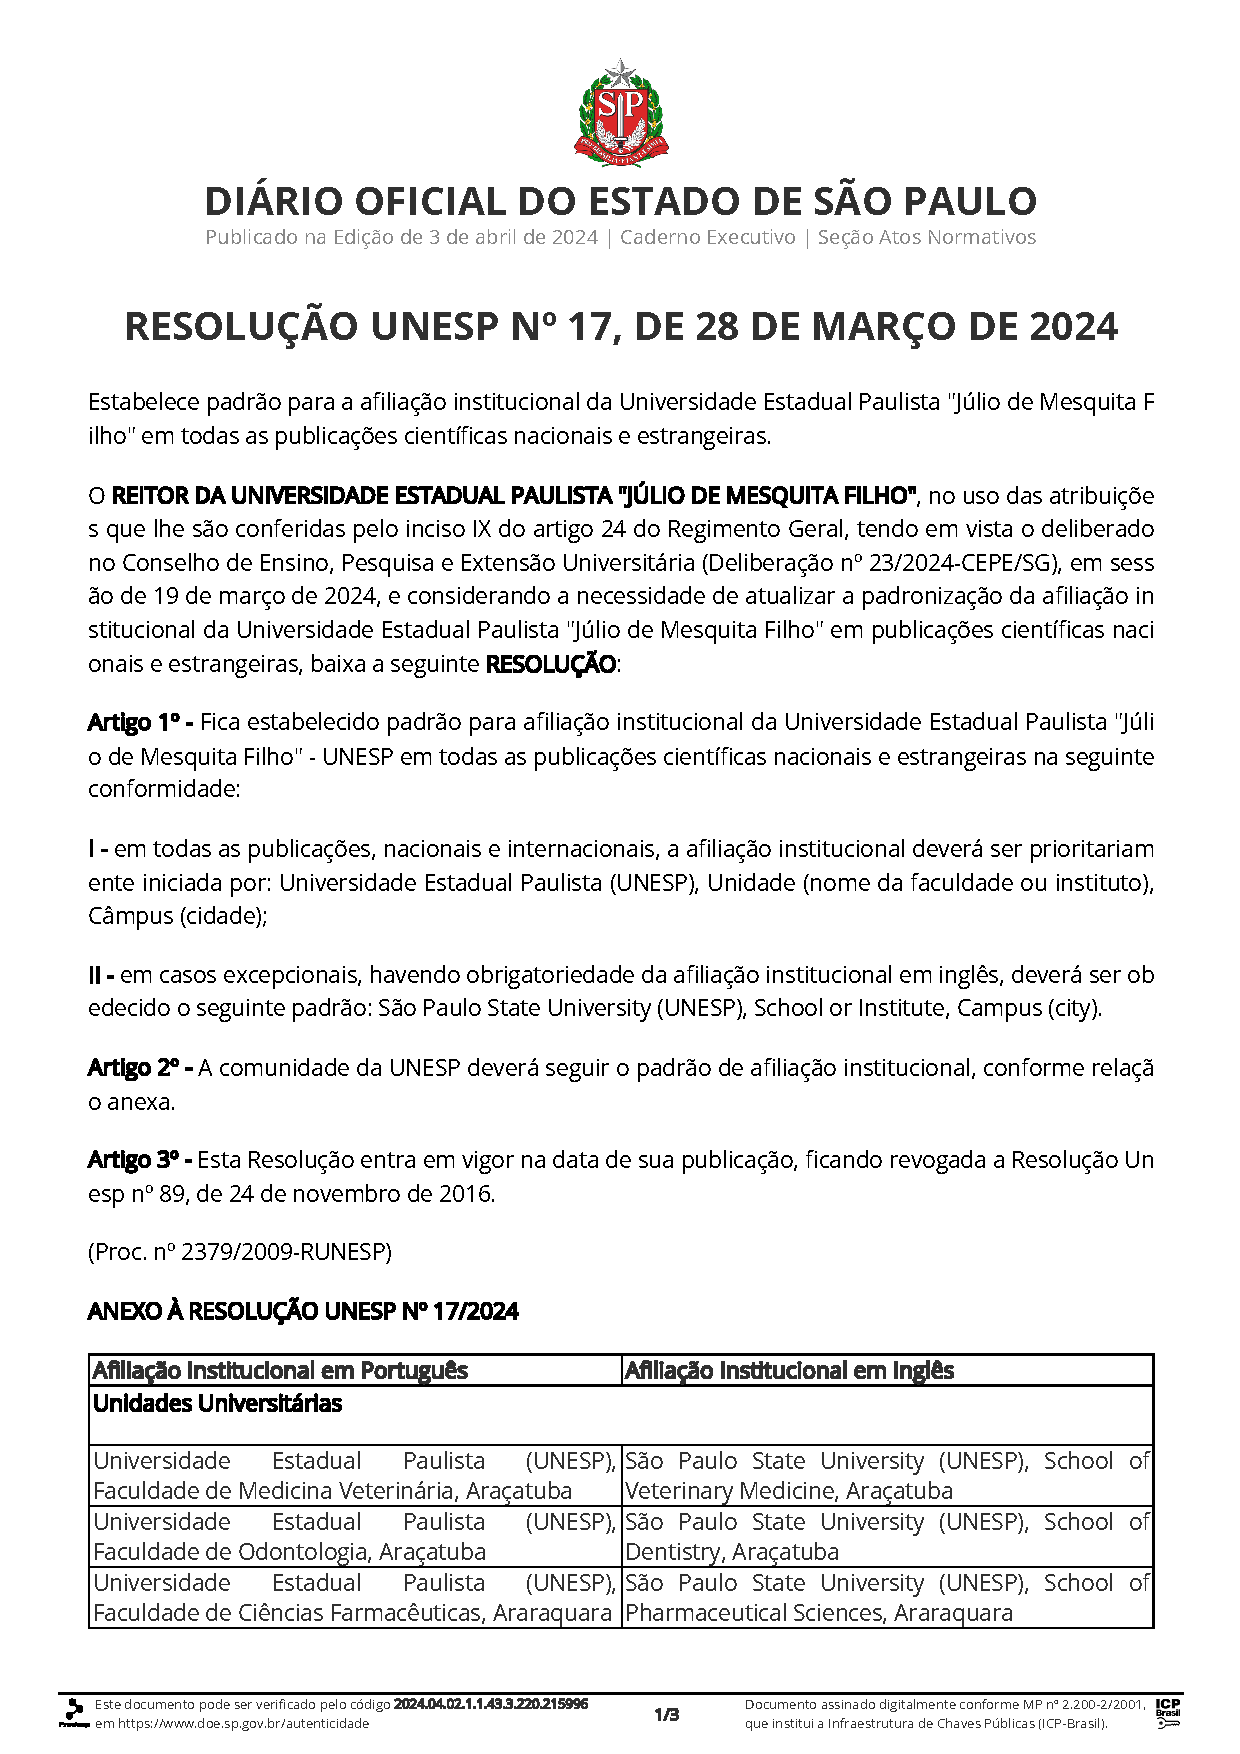
\includepdf[pages=-]{anexos/resolucao_unesp17-2024.pdf}
	
	
\end{anexosenv}
 	\input{partes/09-dados-curriculares.tex}
  	
  	
\end{document}

